% Pollis drill-down: Automatic Transcription, reading manuscripts and early printed books with a model: the phases of a
% transcription, from the page image to the text and its evaluation, the models and methods behind each, the corpora
% they are trained on, and what Explore > Transcription does in Pollis (27 November 2026).
% Compile with: latexmk -pdf workflow_transcription.tex
% Shared look for the one-page Pollis workflow handouts (same fonts and colours as the brochure).
\documentclass[10pt,a4paper]{article}

\usepackage[a4paper,left=17mm,right=17mm,top=14mm,bottom=16mm,footskip=8mm]{geometry}
\usepackage[T1]{fontenc}
\usepackage[default,semibold]{sourcesanspro}
\usepackage{microtype}
\usepackage{graphicx}
\usepackage[table]{xcolor}
\usepackage{tikz}
\usepackage[most]{tcolorbox}
\usepackage{fontawesome5}
\usepackage{enumitem}
\usepackage{fancyhdr}
\usepackage[hidelinks]{hyperref}

\graphicspath{{images/}}

% ---------------------------------------------------------------- colours (as in the brochure)
\definecolor{navy}{HTML}{1C3A5E}
\definecolor{pblue}{HTML}{3B78B5}
\definecolor{amber}{HTML}{F2B33D}
\definecolor{deepamber}{HTML}{D9902A}
\definecolor{pale}{HTML}{EEF3F9}
\definecolor{ink}{HTML}{2A2F36}
\definecolor{logonavy}{HTML}{173D63}
\definecolor{logodark}{HTML}{C98A1E}
\definecolor{logoamber}{HTML}{F2B446}
\definecolor{logocream}{HTML}{FEEFD2}
\definecolor{soft}{HTML}{5E6773}
\color{ink}

\setlength{\parindent}{0pt}
\setlength{\parskip}{3pt}
\setlist{nosep,leftmargin=*,itemsep=2pt}

\pagestyle{fancy}
\fancyhf{}
\renewcommand{\headrulewidth}{0pt}
\fancyfoot[L]{\footnotesize\color{soft}\textbf{Pollis}\enspace Bright Insights through Exploration, Modelling, Simulation and Optimisation}
\fancyfoot[R]{\footnotesize\color{soft}github.com/saragga/pollis/releases/latest}

% The Pollis logo, redrawn so it prints sharply at any size
\newcommand{\pollislogo}[1]{%
  \begin{tikzpicture}[x=#1/512,y=-#1/512,baseline=(current bounding box.center)]
    \fill[logonavy] (0,0) rectangle (512,512);
    \fill[logodark] (36,422) -- (104,256) -- (172,422) -- cycle;
    \fill[logoamber] (104,422) -- (203,180) -- (302,422) -- cycle;
    \fill[logocream] (203,422) -- (339,89) -- (476,422) -- cycle;
  \end{tikzpicture}}

% Top of the page: logo, name, kind of document (Workflow unless given, e.g. [Drill-Down]) and its subject;
% then the question and a one-line promise
\newcommand{\workflowhead}[4][Workflow]{%
  \thispagestyle{fancy}%
  \begin{minipage}[c]{13mm}\pollislogo{11mm}\end{minipage}%
  \begin{minipage}[c]{\dimexpr\linewidth-13mm\relax}
    {\color{navy}\Large\bfseries Pollis}\enspace{\color{soft}#1}\hfill
    {\color{deepamber}\small\bfseries\MakeUppercase{#2}}
  \end{minipage}\par\vspace{7mm}
  {\color{navy}\fontsize{22}{26}\selectfont\bfseries #3}\par\vspace{4pt}
  {\color{soft}\large #4}\par\vspace{5mm}}

% A menu path: \menu{Explore}{Access Data Libraries}... is written as \path{Explore \gt Access Data Libraries}
\newcommand{\gt}{\,{\color{deepamber}\bfseries ›}\,}
\newcommand{\menupath}[1]{{\footnotesize\bfseries\color{navy}#1}}

% A screenshot if images/<file> exists, otherwise an orange placeholder that says what to capture
\newlength{\shotheight}\setlength{\shotheight}{43mm}
\newcommand{\stepshot}[2]{%
  \IfFileExists{images/#1}{%
    \tcbox[enhanced, colback=black, colframe=black!70, boxrule=0.4pt, arc=2pt,
      left=0pt,right=0pt,top=0pt,bottom=0pt, boxsep=0pt, halign=center]{%
      \includegraphics[width=\dimexpr\linewidth-1pt\relax,height=\shotheight,keepaspectratio]{#1}}}{%
    \begin{tcolorbox}[enhanced, colback=white, colframe=orange!80, boxrule=0.6pt, arc=2pt,
      height=\shotheight, valign=center, halign=center, left=6pt, right=6pt]
      {\color{orange}\Large\faCamera}\par\smallskip
      {\color{orange}\footnotesize\bfseries Screenshot: #2}\par\smallskip
      {\color{orange!80!black}\scriptsize images/#1}
    \end{tcolorbox}}}

% One step: number, title, menu path, image file, what to capture, what it means
\newcommand{\step}[6]{%
  \begin{tcolorbox}
    {\color{deepamber}\Large\bfseries #1}\enspace{\color{navy}\large\bfseries #2}\par\vspace{1pt}
    \menupath{#3}\par\vspace{4pt}
    \stepshot{#4}{#5}\par\vspace{3pt}
    {\small #6}
  \end{tcolorbox}}

\newenvironment{steps}{%
  \begin{tcbraster}[raster columns=2, raster equal height=rows, raster column skip=4mm,
    raster row skip=4mm, enhanced, colback=pale, colframe=pale, boxrule=0pt, sharp corners,
    left=6pt,right=6pt,top=6pt,bottom=6pt, fontupper=\raggedright]}{\end{tcbraster}}

% Boxes for the bottom of the page
\newtcolorbox{pbox}[2][]{enhanced, colback=pale, colframe=amber, boxrule=0pt,
  leftrule=3pt, sharp corners, left=7pt, right=7pt, top=6pt, bottom=6pt,
  fontupper=\small\raggedright, before upper={{\color{navy}\normalsize\bfseries #2}\par\smallskip}, #1}
\newtcolorbox{nbox}[1][]{enhanced, colback=navy, colframe=navy, boxrule=0pt,
  sharp corners, left=8pt, right=8pt, top=6pt, bottom=6pt, coltext=white,
  fontupper=\small\raggedright, #1}

% A Next Steps item inside the bottom boxes
\newcommand{\nsitem}[2]{\item[\color{deepamber}\faChevronRight] \textbf{#1}: #2}

% Citations: \dcite{key}{Breiman (2001)} links to its entry \dref{key}{...} in the References, keyed as in pollis.bib
\newcommand{\dcite}[2]{\hyperlink{ref:#1}{\color{pblue}#2}}
\newcommand{\dref}[2]{\raisebox{1.1em}[0pt][0pt]{\hypertarget{ref:#1}{}}#2\par}
\newcommand{\ddoi}[1]{\href{https://doi.org/#1}{\color{pblue}doi:#1}}
\newcommand{\references}{\section*{References}\addcontentsline{toc}{section}{References}\footnotesize\raggedright\setlength{\parskip}{3pt}}

% The page of each heading, for Ask Pollis
% Pollis: the page of each heading, for Ask Pollis. A document that inputs this file, at the end of its preamble, writes
% <jobname>.labels beside its PDF, a line page|level|heading for each heading, the page counted from the first, the
% cover, as 1. compile_documents.jl copies it to ~/.pollis/documents, and ask_index.jl cuts the document into passages
% under its headings with it. \asklabel{1}{Title} marks a topic or a page, \asklabel{2}{Title} a heading inside it; the
% sections and subsections of a document that has them are marked as they go into its contents. A package vignette
% inputs it before its \documentclass (compile_vignette.jl), so the contents are taken over when the document begins,
% after the packages have taken them over. Read a second time, as by a copy of a document for Edit the LaTeX Source,
% which inputs it as resources/ask_labels when Pollis has put it in already (document_source.jl), it does nothing.
\ifdefined\asklabel\endinput\fi
\makeatletter
\newwrite\pollis@labels
\immediate\openout\pollis@labels=\jobname.labels
\newcommand{\asklabel}[2]{\write\pollis@labels{\the\ReadonlyShipoutCounter|#1|\unexpanded{#2}}}
\def\pollis@toc{toc}
\newcommand{\pollis@contentsline}[3]{%
  \def\pollis@file{#1}%
  \ifx\pollis@file\pollis@toc\asklabel{#2}{#3}\fi
  \pollis@addcontentsline{#1}{#2}{#3}}
% The headings of the New Methods style of the vignettes, \nmsection and \nmsub, which go into no contents
\def\pollis@asksection#1{\pollis@nmsection{#1}\asklabel{1}{#1}}
\def\pollis@asksub#1{\pollis@nmsub{#1}\asklabel{2}{#1}}
\AddToHook{begindocument/end}{%
  \let\pollis@addcontentsline\addcontentsline\let\addcontentsline\pollis@contentsline
  \ifdefined\nmsection\let\pollis@nmsection\nmsection\let\nmsection\pollis@asksection\fi
  \ifdefined\nmsub\let\pollis@nmsub\nmsub\let\nmsub\pollis@asksub\fi}
\makeatother



\usepackage{titlesec}
\usepackage{tabularx}
\usepackage{booktabs}
\usepackage{listings}
\usetikzlibrary{positioning,arrows.meta,calc,fit,backgrounds}

\fancyhf{}
\fancyfoot[L]{\footnotesize\color{soft}\textbf{Pollis}\enspace Drill-down: Automatic Transcription}
\fancyfoot[R]{\footnotesize\color{soft}\thepage}

\titleformat{\section}{\color{navy}\large\bfseries}{\color{deepamber}\thesection}{0.6em}{}
\titleformat{\subsection}{\color{navy}\normalsize\bfseries}{\color{deepamber}\thesubsection}{0.5em}{}
\titlespacing*{\section}{0pt}{12pt}{4pt}
\titlespacing*{\subsection}{0pt}{8pt}{2pt}
\setlength{\parskip}{4pt}

\lstset{basicstyle=\ttfamily\footnotesize, columns=fullflexible, keepspaces=true, breaklines=true,
  backgroundcolor=\color{pale}, frame=leftline, rulecolor=\color{amber}, framerule=2pt, xleftmargin=6pt,
  framexleftmargin=6pt, aboveskip=4pt, belowskip=4pt, upquote=true, tabsize=2}

\usepackage{xurl}
\newcommand{\file}[1]{{\small\nolinkurl{#1}}}
\newcolumntype{L}{>{\raggedright\arraybackslash}X}
\newcommand{\ui}[1]{\textbf{#1}}

\begin{document}

\workflowhead[Drill-Down]{Automatic Transcription}
  {Reading manuscripts with a model}
  {The phases of a transcription, from the page image to the text, the models and methods behind each, and the
   corpora they learn from.}

\begin{nbox}
{\color{amber}\bfseries Drill-down.}\enspace
Automatic transcription, also called handwritten text recognition (HTR) or automatic text recognition (ATR), reads
the text of a manuscript or an early printed book from images of its pages. It goes through several phases: the page
is photographed, its text lines are found, each line is cut out and read by a model, and the text read is decoded,
combined with that of other models, normalised and measured against a transcription made by hand.

This drill-down describes each phase and the methods behind it (\S\ref{sec:glance} to \S\ref{sec:evaluation}), the
transcriptions and corpora models are trained on (\S\ref{sec:training}), and what the Transcription page, in
\ui{Explore}\gt\ui{Transcription}, does in Pollis (\S\ref{sec:pollis}).
\end{nbox}

{\setlength{\parskip}{0pt}\tableofcontents}

\section{What it is for}\label{sec:why}
\begin{itemize}
  \item \textbf{Most manuscripts have never been transcribed.} Libraries and archives have put millions of pages
    online as images, and only a small part of them has been read and edited. A model makes a first transcription
    of a whole collection, which can then be searched, compared and corrected.
  \item \textbf{A transcription by hand is slow and needs training in palaeography.} The scripts, abbreviations and
    languages of the Middle Ages change from one century, region and scribe to the next.
  \item \textbf{The same model reads many manuscripts.} A model trained on transcriptions that follow the same
    guidelines, across centuries, languages and scripts, reads manuscripts it has not seen, and can be fine-tuned
    on a few pages of a new one.
\end{itemize}

\section{The phases at a glance}\label{sec:glance}
The phases go from top to bottom; beside each are the models and methods that carry it out. The phases in navy are
those the Transcription page of Pollis carries out (\S\ref{sec:pollis}). Ground truth, at the bottom, is a
transcription made by hand: the models of layout analysis and recognition are trained on it, and evaluation measures
the text read against it.

\begin{center}
\makebox[\linewidth][c]{%
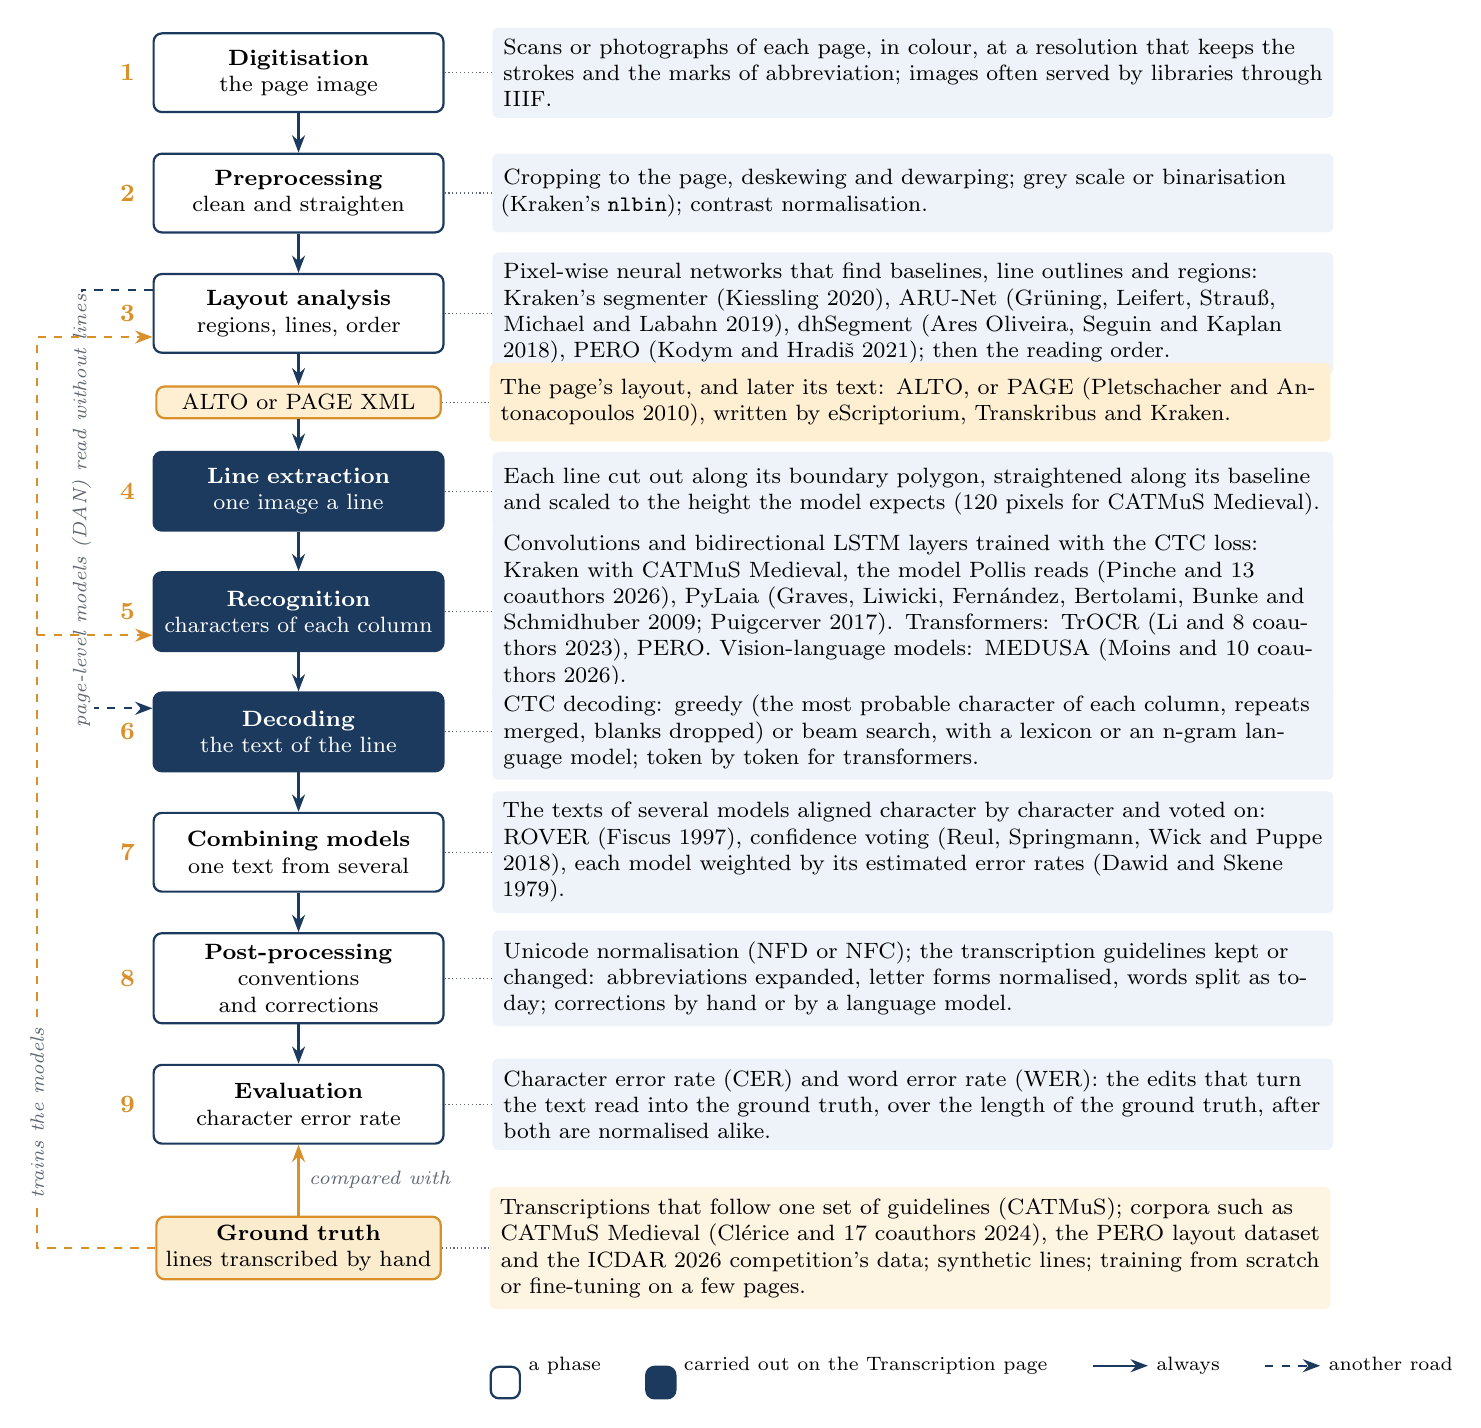
\begin{tikzpicture}[font=\footnotesize,
  phase/.style={draw=navy, line width=0.8pt, rounded corners=3pt, fill=white, align=center, text width=34mm,
    minimum height=10mm, inner sep=4pt},
  inpollis/.style={phase, fill=navy, text=white},
  method/.style={draw=none, fill=pale, rounded corners=2pt, align=left, text width=104mm, minimum height=10mm,
    inner sep=4pt, anchor=west},
  store/.style={draw=deepamber, line width=0.8pt, rounded corners=3pt, fill=logocream, align=center, text width=34mm,
    inner sep=3pt},
  flow/.style={-{Stealth[length=2.2mm]}, line width=0.8pt, draw=navy},
  optflow/.style={flow, dashed},
  tie/.style={draw=soft, line width=0.4pt, densely dotted},
  num/.style={font=\bfseries\small, text=deepamber, anchor=east}]

  % ---------- the phases ----------
  \node[phase] (p1) at (0,0) {\textbf{Digitisation}\\the page image};
  \node[phase, below=5mm of p1] (p2) {\textbf{Preprocessing}\\clean and straighten};
  \node[phase, below=5mm of p2] (p3) {\textbf{Layout analysis}\\regions, lines, order};
  \node[store, below=4mm of p3] (xml) {ALTO or PAGE XML};
  \node[inpollis, below=4mm of xml] (p4) {\textbf{Line extraction}\\one image a line};
  \node[inpollis, below=5mm of p4] (p5) {\textbf{Recognition}\\characters of each column};
  \node[inpollis, below=5mm of p5] (p6) {\textbf{Decoding}\\the text of the line};
  \node[phase, below=5mm of p6] (p7) {\textbf{Combining models}\\one text from several};
  \node[phase, below=5mm of p7] (p8) {\textbf{Post-processing}\\conventions and corrections};
  \node[phase, below=5mm of p8] (p9) {\textbf{Evaluation}\\character error rate};
  \node[store, below=9mm of p9, text width=34mm, fill=amber!25] (gt) {\textbf{Ground truth}\\lines transcribed by hand};

  \foreach \i/\n in {p1/1, p2/2, p3/3, p4/4, p5/5, p6/6, p7/7, p8/8, p9/9} {\node[num] at ($(\i.west)+(-1mm,0)$) {\n};}

  \draw[flow] (p1) -- (p2);
  \draw[flow] (p2) -- (p3);
  \draw[flow] (p3) -- (xml);
  \draw[flow] (xml) -- (p4);
  \draw[flow] (p4) -- (p5);
  \draw[flow] (p5) -- (p6);
  \draw[flow] (p6) -- (p7);
  \draw[flow] (p7) -- (p8);
  \draw[flow] (p8) -- (p9);
  \draw[flow, draw=deepamber] (gt) -- node[right, text=soft, font=\scriptsize\itshape] {compared with} (p9);

  % ---------- the methods ----------
  \node[method] (m1) at ($(p1.east)+(6mm,0)$) {Scans or photographs of each page, in colour, at a resolution that keeps the
    strokes and the marks of abbreviation; images often served by libraries through IIIF.};
  \node[method] (m2) at ($(p2.east)+(6mm,0)$) {Cropping to the page, deskewing and dewarping; grey scale or binarisation
    (Kraken's \texttt{nlbin}); contrast normalisation.};
  \node[method] (m3) at ($(p3.east)+(6mm,0)$) {Pixel-wise neural networks that find baselines, line outlines and regions:
    Kraken's segmenter (Kiessling 2020), ARU-Net (Grüning, Leifert, Strauß, Michael and Labahn 2019), dhSegment
    (Ares Oliveira, Seguin and Kaplan 2018), PERO (Kodym and Hradiš 2021); then the reading order.};
  \node[method, fill=logocream] (mx) at ($(xml.east)+(6mm,0)$) {The page's layout, and later its text: ALTO, or PAGE
    (Pletschacher and Antonacopoulos 2010), written by eScriptorium, Transkribus and Kraken.};
  \node[method] (m4) at ($(p4.east)+(6mm,0)$) {Each line cut out along its boundary polygon, straightened along its
    baseline and scaled to the height the model expects (120 pixels for CATMuS Medieval).};
  \node[method] (m5) at ($(p5.east)+(6mm,0)$) {Convolutions and bidirectional LSTM layers trained with the CTC loss:
    Kraken with CATMuS Medieval, the model Pollis reads (Pinche and 13 coauthors 2026), PyLaia (Graves, Liwicki,
    Fernández, Bertolami, Bunke and Schmidhuber 2009; Puigcerver 2017). Transformers: TrOCR (Li and 8 coauthors 2023),
    PERO. Vision-language models: MEDUSA (Moins and 10 coauthors 2026).};
  \node[method] (m6) at ($(p6.east)+(6mm,0)$) {CTC decoding: greedy (the most probable character of each column, repeats
    merged, blanks dropped) or beam search, with a lexicon or an n-gram language model; token by token for
    transformers.};
  \node[method] (m7) at ($(p7.east)+(6mm,0)$) {The texts of several models aligned character by character and voted on:
    ROVER (Fiscus 1997), confidence voting (Reul, Springmann, Wick and Puppe 2018), each model weighted by its estimated error
    rates (Dawid and Skene 1979).};
  \node[method] (m8) at ($(p8.east)+(6mm,0)$) {Unicode normalisation (NFD or NFC); the transcription guidelines kept or
    changed: abbreviations expanded, letter forms normalised, words split as today; corrections by hand or by a
    language model.};
  \node[method] (m9) at ($(p9.east)+(6mm,0)$) {Character error rate (CER) and word error rate (WER): the edits that turn
    the text read into the ground truth, over the length of the ground truth, after both are normalised alike.};
  \node[method, fill=amber!15] (mg) at ($(gt.east)+(6mm,0)$) {Transcriptions that follow one set of guidelines
    (CATMuS); corpora such as CATMuS Medieval (Clérice and 17 coauthors 2024), the PERO layout dataset and the
    ICDAR 2026 competition's data; synthetic lines; training from scratch or fine-tuning on a few pages.};

  \foreach \i in {1,...,9} {\draw[tie] (p\i.east) -- (m\i.west);}
  \draw[tie] (xml.east) -- (mx.west);
  \draw[tie] (gt.east) -- (mg.west);

  % ---------- page-level models skip the lines ----------
  \draw[optflow] ($(p3.west)+(0,3mm)$) -- ++(-9mm,0) coordinate (c1) |- ($(p6.west)+(0,3mm)$);
  \node[rotate=90, font=\scriptsize\itshape, text=soft, fill=white, inner sep=1pt] at ($(c1)!0.5!(c1 |- p6.west)$)
    {page-level models (DAN) read without lines};

  % ---------- training ----------
  \draw[optflow, draw=deepamber] (gt.west) -- ++(-15mm,0) coordinate (c2) |- ($(p3.west)+(0,-3mm)$);
  \coordinate (t5) at ($(p5.west)+(0,-3mm)$);
  \draw[optflow, draw=deepamber] (c2 |- t5) -- (t5);
  \node[rotate=90, font=\scriptsize\itshape, text=soft, fill=white, inner sep=1pt] at ($(c2 |- p8.west)!0.5!(c2 |- gt.west)$)
    {trains the models};

  % ---------- legend ----------
  \node[below=6mm of mg.south west, anchor=north west, inner sep=0, font=\scriptsize] {%
    \tikz[baseline=-0.6ex]\node[phase, text width=3mm, minimum height=4mm, inner sep=1pt] {}; a phase\qquad
    \tikz[baseline=-0.6ex]\node[inpollis, text width=3mm, minimum height=4mm, inner sep=1pt] {}; carried out on the
    Transcription page\qquad
    \tikz[baseline=-0.6ex]\draw[flow] (0,0) -- (7mm,0); always\qquad
    \tikz[baseline=-0.6ex]\draw[optflow] (0,0) -- (7mm,0); another road};
\end{tikzpicture}}
\end{center}

Two roads differ from the one drawn. A \emph{page-level} model, such as the Document Attention Network of
\dcite{CCP2023a}{Coquenet, Chatelain and Paquet (2023)}, reads the whole page and gives its text, with tags for its
parts, without finding lines first. A \emph{platform} such as eScriptorium
(\dcite{KTSS2019a}{Kiessling, Tissot, Stokes and Stökl Ben Ezra (2019)}) or Transkribus
(\dcite{KCHM2017a}{Kahle, Colutto, Hackl and Mühlberger (2017)}) carries out phases 2 to 6 on a server, keeps the
pages, their layout and text, and lets people correct both and train models on the corrections.

\section{Digitisation and preprocessing}\label{sec:image}
The transcription can only be as good as the image. A page is photographed or scanned whole, in colour, at a
resolution at which the smallest marks, such as a superscript letter or the stroke through a \emph{p} that makes it
\emph{per}, are several pixels wide. Many libraries serve their images through IIIF, from which a page can be fetched
at the size wanted.

Preprocessing makes the page easier to read for what follows: cropping it to the page, turning it so its lines are
level (deskewing), flattening the curve of a bound volume (dewarping), and turning it into grey or into black and
white (binarisation). Kraken's binarisation is \texttt{nlbin}. The CATMuS Medieval model reads each line in grey.

\section{Layout analysis}\label{sec:layout}
Layout analysis, also called segmentation, finds what is on the page and where: the regions (columns, glosses,
initials, illustrations), the text lines in each, and the order in which they are read.

\subsection{Baselines and boundaries}
Each text line is given by two shapes on the image:
\begin{itemize}
  \item its \textbf{baseline}, the line its letters stand on, as a polyline of points;
  \item its \textbf{boundary}, the polygon around the line, from the tops of the tallest letters to the bottoms of the
    descenders.
\end{itemize}
A baseline follows a line that curves or slopes, which a rectangle around it cannot. The cBAD competition of ICDAR
2017 was a competition on baseline detection.

\subsection{The methods}
Today's segmenters are neural networks that label each pixel of the page: on a baseline, between lines, in a region of
a given kind, or none of these. The baselines and polygons are then traced from the labels.
\begin{itemize}
  \item \textbf{Kraken's segmenter}, \dcite{Kie2020a}{Kiessling (2020)}, predicts baselines and regions of the
    kinds it is trained on, and can be retrained for a new layout.
  \item \textbf{ARU-Net}, of \dcite{GLSML2019a}{Grüning, Leifert, Strauß, Michael and Labahn (2019)}, labels
    baselines and the ends of lines, then clusters them into baselines; it is trainable from fewer than 50 pages.
  \item \textbf{dhSegment}, of \dcite{ASK2018a}{Ares Oliveira, Seguin and Kaplan (2018)}, is one network for many
    tasks: the page, its baselines, its regions and its illustrations.
  \item \textbf{PERO}, of \dcite{KH2021a}{Kodym and Hradiš (2021)}, predicts with each baseline the height of its
    line and the boundaries of the text blocks, and handles text written in several orientations.
\end{itemize}

\subsection{ALTO and PAGE files}
The layout is written to an XML file beside the image, which later phases read and complete with the text:
\textbf{ALTO}, of the Library of Congress, or \textbf{PAGE}, of
\dcite{PA2010a}{Pletschacher and Antonacopoulos (2010)}, which also records how the image was cleaned. Both give
for each text line its baseline, its polygon and, once read, its text. eScriptorium, Transkribus and Kraken write
both; so do most corpora of manuscripts with their ground truth.

\section{Line extraction}\label{sec:lines}
A line recognition model reads one line at a time, as an image of fixed height. Each line is cut out of the page
along its boundary polygon, everything outside the polygon left blank, straightened along its baseline, so that a
sloping or curved line becomes level, and scaled to the height the model was trained on: 120 pixels, in grey, for
CATMuS Medieval. The way a line is cut matters: a model reads best the lines cut as its training lines were cut.

\section{Recognition}\label{sec:recognition}
Recognition gives, for each position along the line, the probability of each character of the model's alphabet.

\subsection{Convolutional and recurrent networks}
The most used models read the line image from left to right as a sequence of columns. Convolutional layers find the
shapes of strokes; bidirectional long short-term memory (LSTM) layers, of
\dcite{HS1997a}{Hochreiter and Schmidhuber (1997)}, read the sequence in both directions, so that each column is read
with what comes before and after it. \dcite{GLFBB...2009a}{Graves, Liwicki, Fernández, Bertolami, Bunke and
Schmidhuber (2009)} showed such networks reading unconstrained handwriting better than hidden Markov models, and
\dcite{Pui2017a}{Puigcerver (2017)} showed that convolutions with one-dimensional recurrent layers do as well as
multidimensional ones, faster, and that distorting the training lines at random improves them. Kraken and PyLaia
are models of this kind.

Such a model needs no position of each character in its training lines: it is trained with the loss of
connectionist temporal classification (CTC), of \dcite{GFGS2006a}{Graves, Fernández, Gomez and Schmidhuber (2006)},
which sums over every way of placing the characters of the line's text along its columns, with a \emph{blank} for
the columns between them.

\subsection{Kraken and CATMuS Medieval}
Kraken is an engine of automatic text recognition for historical documents, written in Python
(\dcite{Kie2019a}{Kiessling (2019)}; \dcite{Kie2025a}{Kiessling (2025)}). Its recognition models are of the kind
above, and CATMuS Medieval, of \dcite{PCVCC...2026a}{Pinche and 13 coauthors (2026)}, is one of them, trained on the
CATMuS Medieval corpus (\S\ref{sec:training}). It is the model Pollis reads, through MedievalATR.jl (\S\ref{sec:pollis}).

\begin{center}\small
\begin{tabularx}{\linewidth}{@{}p{0.28\linewidth}L@{}}
\toprule
\textbf{CATMuS Medieval 1.6.2} & \\
\midrule
Input & A line image in grey, scaled to 120 pixels high \\
Network & Four convolutions, three bidirectional LSTM layers of 200 units, 252 outputs, trained with the CTC loss \\
Decoding & Greedy CTC decoding \\
Languages of its training data & Old and Middle French, Latin, Spanish and other languages of Spain, Italian \\
Transcription & Graphematic: abbreviations not expanded, each diacritic a character of its own (NFD) \\
File & \file{catmus-medieval-1.6.0.mlmodel}, 16 MB, on Zenodo, CC BY 4.0 \\
ICDAR 2026 competition & As CATMuS Medieval 1.6, the organisers' baseline, with no adaptation: a character error
  rate of 9.30\% on Task 1, 7.92\% on Task 2 and 25.92\% on Task 3, 7th of 13 entries on Task 1 and 5th of 10 on
  Tasks 2 and 3 (\S\ref{sec:evaluation}) \\
\bottomrule
\end{tabularx}
\end{center}

\subsection{Transformers and vision-language models}
\textbf{TrOCR}, of \dcite{LLCCL...2023a}{Li and 8 coauthors (2023)}, reads a line with a transformer
(\dcite{VSPUJ...2017a}{Vaswani and 7 coauthors (2017)}) for the image and another that writes the text, both
pre-trained, the first on images and the second on text, then fine-tuned on lines. \textbf{Vision-language models},
trained on images and text of every kind, can be fine-tuned to transcribe lines.

\subsection{The three highest scorers of the ICDAR 2026 competition}
The three systems with the lowest error rates in the ICDAR 2026 competition (\S\ref{sec:evaluation}) read lines with
transformers, as their teams describe them on the competition's results page.
\begin{itemize}
  \item \textbf{PERO}, built on the pero-ocr framework, whose layout analysis \dcite{KH2021a}{Kodym and Hradiš (2021)}
    describe, first refines the outline of each line with a layout model trained on the PERO layout dataset, then reads it, scaled to 48 pixels high, with an
    encoder--decoder transformer that writes the text character by character: a VGG-like convolutional backbone and six
    transformer layers in the encoder, six in the decoder. It was trained on the competition's data and on other
    corpora, among them CATMuS Medieval and TRIDIS, with blurring, noise, distortions and masking. Its decoding keeps
    the 16 most probable texts, from which it builds a confusion network and takes its most probable path.
  \item \textbf{The Swedish National Archives' AI lab} fine-tuned TrOCR on the competition's data, from a model already
    trained on historical Swedish, with two changes: line images of $192 \times 1024$ pixels instead of
    $384 \times 384$, more detail along the line, and a vocabulary of bytes instead of word pieces, which the team
    expected to depend less on the patterns of the training languages and so to read unseen languages better.
  \item \textbf{MEDUSA}, of the École nationale des chartes, fine-tunes the Qwen 3.5 vision-language model with LoRA,
    in stages: on lines transcribed under other guidelines (Gold), then on lines that follow the CATMuS guidelines
    (Platinum), some 643,000 lines in all from more than twenty repositories. Version 0.1, the one entered in the
    competition, is described in the system report of \dcite{MCCCG...2026a}{Moins and 10 coauthors (2026)}; version
    0.2 adds a first stage on synthetic lines made from text-only corpora (Silver), as
    \dcite{MHCCC...2026a}{Moins and 10 coauthors (2026)} describe. Both are published on Hugging Face, each in a model
    of 4 and one of 9 billion parameters, under CC BY 4.0. Its authors name the control of hallucinated
    transcriptions, fluent text not grounded in the image, as one of the challenges of such models.
\end{itemize}

\section{Decoding}\label{sec:decoding}
Decoding turns the probabilities into text.
\begin{itemize}
  \item \textbf{Greedy decoding} of CTC takes the most probable character of each column, merges repeated
    characters and drops the blanks. It is fast and needs nothing but the model.
  \item \textbf{Beam search} keeps the most probable texts so far at each column, and can weigh them with a lexicon
    or a language model of the language, such as an $n$-gram model (\dcite{Kat1987a}{Katz (1987)};
    \dcite{CG1999a}{Chen and Goodman (1999)}). A language model helps where the image is unclear, and can mislead
    where a manuscript's spelling is not that of the texts it was built from.
  \item A \textbf{transformer} or a vision-language model writes its text token by token, each token chosen from
    those before it.
\end{itemize}

\section{Combining models}\label{sec:combining}
Models trained differently make different errors, so the text of several models, put together, can have fewer
errors than that of any of them.
\begin{itemize}
  \item \textbf{ROVER}, of \dcite{Fis1997a}{Fiscus (1997)}, made for speech recognition, aligns the outputs of
    several recognisers into one network of words and takes, at each place, the word most of them give, or the one
    with the best confidence.
  \item \dcite{RSWP2018a}{Reul, Springmann, Wick and Puppe (2018)} trained several models of early printed books,
    each on a part of the ground truth, and voted on their texts character by character, using each character's
    confidence and its alternatives.
  \item The model of \dcite{DS1979a}{Dawid and Skene (1979)}, made for observers who rate patients, estimates by the
    EM algorithm how often each observer errs and in which way, without knowing the true answer, and weighs each
    one's answer by it. Applied to recognisers, it trusts each model as much as its estimated error rates allow.
\end{itemize}
Voting needs the texts aligned: character by character on the same line, which is why each model is given the same
lines, cut alike.

\section{Transcription conventions and post-processing}\label{sec:conventions}
A transcription follows guidelines that say how each sign is written down, and models learn those of their training
data.
\begin{itemize}
  \item \textbf{Graphematic} or \textbf{diplomatic}: the letters and signs as written, abbreviations not expanded.
    CATMuS Medieval reads so: a mark of abbreviation, such as a tilde, is a character of its own, after the letter it
    stands on (Unicode form NFD).
  \item \textbf{Normalised}: abbreviations expanded, letter forms such as long and round \emph{s} made one, words
    split as today, punctuation modernised, as for a reading edition.
\end{itemize}
Post-processing brings the text read to the guidelines wanted: Unicode normalisation (NFD or NFC), a check that every
character is one the guidelines allow, abbreviations expanded, and corrections, by hand or with a language model,
whose changes are best kept apart from the text read so that they can be checked.

\section{Evaluation}\label{sec:evaluation}
A model is measured on lines it was not trained on, against their ground truth.
\begin{itemize}
  \item The \textbf{character error rate} (CER) is the least number of characters inserted, deleted and substituted
    to turn the text read into the ground truth (their Levenshtein distance), divided by the number of characters
    of the ground truth.
  \item The \textbf{word error rate} (WER) is the same on words.
\end{itemize}
Both are computed over all the lines of a test set together, or for each language and then averaged. The two texts
must be normalised alike first: the same Unicode form, the same treatment of spaces, the same characters allowed.
A difference of normalisation alone changes the rate.

\subsection{The ICDAR 2026 competition}
The ICDAR 2026 Competition on Multilingual Medieval Handwriting Recognition (CMMHWR26), organised by
\dcite{CK2026a}{Clérice and Kiessling (2026)}, measured how well models read manuscripts in languages they were and
were not trained on, in three tasks:
\begin{enumerate}
  \item \textbf{Multilingual recognition}: manuscripts in the eight Romance languages of the training set, Castilian,
    Catalan, French, Galician, Italian, Latin, Navarrese and Venetian;
  \item \textbf{Within the language family}: manuscripts in Occitan, a Romance language absent from the training set;
  \item \textbf{Across language families}: manuscripts in Czech, in hands like those of the training set.
\end{enumerate}
Task 1 is scored by the character error rate averaged over French, Latin and Spanish. Teams could train on data
beyond the competition's training set. Its test set was published first without its transcriptions, for the
competition, then with them, so that any model can be scored on it.

Twelve teams submitted results, all of them to Task 1 and nine to Tasks 2 and 3. The organisers' baseline is Kraken
with the CATMuS Medieval 1.6 model, with no adaptation to the tasks. The table gives each team's best submission, with
its method as the team describes it, in the order of Task 1; a dash marks a task the team did not enter.

\begin{center}\footnotesize
\begin{tabularx}{\linewidth}{@{}p{0.25\linewidth}Lrrr@{}}
\toprule
 & & \multicolumn{3}{c}{\textbf{CER (\%)}}\\
\cmidrule(l){3-5}
\textbf{Team} & \textbf{Method} & \textbf{Task 1} & \textbf{Task 2} & \textbf{Task 3}\\
\midrule
PERO & Encoder--decoder transformer writing characters (\S\ref{sec:recognition}), lines refined by a layout model trained on the PERO layout
  dataset, trained also on CATMuS Medieval, TRIDIS and other corpora & 7.71 & 6.58 & 10.27\\
Swedish National Archives' AI lab & TrOCR with wider line images and a byte-level vocabulary (\S\ref{sec:recognition}), from a model trained on
  historical Swedish & 7.73 & 6.83 & 23.39\\
École nationale des chartes & MEDUSA 0.1: the Qwen 3.5 vision-language model of 9 billion parameters, fine-tuned with
  LoRA in stages on Gold and Platinum lines (\S\ref{sec:recognition}) & 8.03 & 5.01 & 10.79\\
PRHLT-tS & Convolutions and bidirectional LSTM layers with CTC, decoded with an 8-gram character language model;
  for Task 3, a transformer encoder and a 10-gram model & 8.23 & 7.43 & 25.99\\
FamilySearch \& GGateway & For Task 1, convolutions and LSTM layers with CTC and an $n$-gram language model; for Tasks 2
  and 3, a ResNet with Conformer blocks and two heads, CTC and a transformer decoder & 9.02 & 8.50 & 24.04\\
TeamAnannya & ROVER over three models: five TrOCR models voting, a TrOCR with a vocabulary of its own, and Kraken
  with CATMuS Medieval & 9.09 & 9.56 & 27.17\\
Baseline & Kraken with CATMuS Medieval 1.6, no adaptation & 9.30 & 7.92 & 25.92\\
Teodor Bors & ConvNeXt-V2 encoder and a bidirectional Mamba-2 module, with CTC & 9.61 & 9.71 & 27.38\\
Qianfan-OCR & Qianfan-OCR, a vision-language model of 4 billion parameters, fine-tuned on historical documents & 9.94 &
  -- & --\\
STUDIUM.AI & TrOCR with eight LoRA adapters, one for each language, mixed by a network that predicts the language &
  12.87 & -- & --\\
Devansh Gupta & The Qwen 3.5 vision-language model of 0.8 billion parameters, with a LoRA adapter for each language &
  14.81 & 13.08 & 33.35\\
FLAME University & Kraken's CATMuS Medieval 1.5.0 model, fine-tuned on the training set & 15.48 & 13.74 & 29.04\\
nampfiev1995 & No description & 42.38 & -- & --\\
\midrule
PERO, after the deadline & PERO's production model, a larger transformer & 6.94 & 6.08 & 10.11\\
\bottomrule
\end{tabularx}
\end{center}
{\footnotesize Source: \href{https://cmmhwr26.inria.fr/results/}{\color{pblue}the competition's results page}, which also gives the
word error rates.}

Among the entries made in time, the baseline, Kraken with CATMuS Medieval as it is, ranks in the middle: 7th of 13
on Task 1, and 5th of 10 on Tasks 2 and 3.

The entries carry out the phases of \S\ref{sec:glance} in different ways: language models in decoding (PRHLT-tS,
FamilySearch \& GGateway), voting over models (TeamAnannya), fine-tuning of a Kraken model (FLAME University), and
vision-language models (École nationale des chartes, Qianfan-OCR, Devansh Gupta).

\section{Ground truth and training}\label{sec:training}
Ground truth is a set of page images with their layout and the text of each line transcribed by hand, under one set
of guidelines.

\subsection{Corpora}
\begin{center}\small
\begin{tabularx}{\linewidth}{@{}p{0.27\linewidth}L@{}}
\toprule
\textbf{Corpus} & \textbf{What it holds} \\
\midrule
CATMuS Medieval & The transcriptions of more than 200 manuscripts and incunabula in 10 languages, from the 8th to
  the 16th century, under the CATMuS guidelines, by \dcite{CPVCC...2024a}{Clérice and 17 coauthors (2024)}; the
  data of the CATMuS Medieval model (\dcite{PCVCC...2026a}{Pinche and 13 coauthors (2026)}) \\
ICDAR 2026 competition & The test pages of the three tasks of the competition (\S\ref{sec:evaluation}), with their
  transcriptions, by \dcite{CK2026a}{Clérice and Kiessling (2026)} \\
TRIDIS & About 4,000 pages of documentary manuscripts, registers, charters, proceedings and accounts, from the 12th to
  the 17th century, transcribed semi-diplomatically, by \dcite{Tor2025a}{Torres Aguilar (2025)} \\
PERO layout dataset & Pages of historical documents with their text lines and regions, the layout data of
  \dcite{KH2021b}{Kodym and Hradiš (2021)} \\
MEDUSA's synthetic lines & Line images made from text-only corpora of medieval languages, the Silver data of
  MEDUSA 0.2 \\
\bottomrule
\end{tabularx}
\end{center}

\ui{Explore}\gt\ui{Transcription}\gt\ui{Browse Training Corpora...} lists the first four, with their languages,
transcription, size and licence, each opening at its source.

\subsection{Training and fine-tuning}
A recognition model is trained on line images with their text, for the CTC loss; a segmenter, on page images with
their baselines and regions. Training from scratch needs many thousands of lines; \emph{fine-tuning} starts from a
trained model and needs only a few pages of the new manuscript, since what the first layers have learnt carries over
(\dcite{YCBL2014a}{Yosinski, Clune, Bengio and Lipson (2014)}). Random distortions of the training lines, and
synthetic lines, add variety where the data are few.

\section{Automatic transcription in Pollis}\label{sec:pollis}
The Transcription page, in \ui{Explore}\gt\ui{Transcription}\gt\ui{Transcribe a Page...}, carries out phases 4 to 6 of the diagram on a page
whose layout is already known. It reads each line with MedievalATR.jl, a Julia package that reads the recognition
models of Kraken, in the Julia REPL, without Python.

\subsection{The four steps}
\begin{enumerate}
  \item \textbf{Page}: \ui{Choose a Page File...} chooses the ALTO or PAGE file of the page. The step shows the file,
    the image it names and the number of its text lines.
  \item \textbf{Model}: \ui{CATMuS Medieval 1.6.2}, downloaded from Zenodo (16 MB) the first time it is used, then
    kept, or \ui{A Model File of Your Own}, a Kraken \file{.mlmodel}.
  \item \textbf{Transcribe}: the Julia code that reads every line, which \ui{Transcribe} sends to the Julia REPL. The
    lines are read on the REPL's threads.
  \item \textbf{Text}: the page image with the outline of each line drawn on it, and the text read beside each line;
    pointing to a line shows its outline, and pointing to an outline finds its line. A transcription already in the
    page file is shown under the text read. \ui{Copy Text} copies the text, a line of the page to a line, and
    \ui{Open the Results File} opens the results.
\end{enumerate}

\subsection{The same text as Kraken}
MedievalATR.jl reads a line as Kraken 7.2 reads it: the same lines from ALTO and PAGE files, the line images cut
pixel for pixel as Kraken cuts them, the same network and the same greedy decoding, so the text read on a line is the
text Kraken reads with the same model. A line Kraken cannot read, one without a boundary or whose image is empty, is
read as empty.

\subsection{The Julia code}
The code of step 3, for a page file \file{page.xml}:
\begin{lstlisting}
using MedievalATR
model = load_model(:catmus_medieval)
page = read_page("page.xml")
predictions = recognize(model, page)
write_predictions("page.transcription.json", page, predictions)
\end{lstlisting}

\begin{center}\small
\begin{tabularx}{\linewidth}{@{}p{0.36\linewidth}L@{}}
\toprule
\textbf{Function} & \textbf{What it does} \\
\midrule
\texttt{load\_model(:catmus\_medieval)} & The CATMuS Medieval model, downloaded the first time and checked by its
  SHA-256 checksum \\
\texttt{load\_model(path)} & A Kraken recognition model from its \file{.mlmodel} file \\
\texttt{read\_page(path)} & The image and text lines of an ALTO or PAGE file \\
\texttt{recognize(model, page)} & The text of each line, read on Julia's threads \\
\texttt{write\_predictions(path, page, predictions)} & The results file of step 4 \\
\texttt{cut\_line(image, baseline, boundary)} & The image of one line, straightened along its baseline \\
\bottomrule
\end{tabularx}
\end{center}

\subsection{Files}
\begin{center}\small
\begin{tabularx}{\linewidth}{@{}p{0.30\linewidth}L@{}}
\toprule
\textbf{File} & \textbf{What it is} \\
\midrule
The page file, \file{.xml} & ALTO or PAGE: the image's name and the text lines, read \\
The page image & JPEG, PNG or TIFF, at the path the page file gives, or next to it, read \\
\file{<page>.transcription.json} & Written next to the page file: the image and, for each line, its id, baseline,
  polygon, the text read and the page file's own transcription \\
\file{~/.julia/scratchspaces/.../models} & The CATMuS Medieval model, once downloaded \\
\bottomrule
\end{tabularx}
\end{center}

\section{Menu items}\label{sec:menu}
\begin{center}\small
\begin{tabularx}{\linewidth}{@{}p{0.30\linewidth}L@{}}
\toprule
\textbf{Item} & \textbf{What it does} \\
\midrule
\ui{Explore}\gt\ui{Transcription}\gt\ui{Transcribe a Page...} & Opens the Transcription page, with its four steps
  (\S\ref{sec:pollis}) \\
\ui{Explore}\gt\ui{Transcription}\gt\ui{Browse Training Corpora...} & Opens the Training Corpora page: the corpora of
  \S\ref{sec:training}, each opening at its source \\
\ui{Help}\gt\ui{Documentation}\gt\ui{Drill-downs}\gt\ui{Automatic Transcription} & Opens this drill-down \\
\bottomrule
\end{tabularx}
\end{center}

\references
\dref{ASK2018a}{Ares Oliveira, S., Seguin, B. and Kaplan, F. (2018). dhSegment: A Generic Deep-Learning Approach for Document Segmentation. In \emph{2018 16th International Conference on Frontiers in Handwriting Recognition (ICFHR)}, 7--12. IEEE. \ddoi{10.1109/ICFHR-2018.2018.00011}}
\dref{CG1999a}{Chen, S.\,F. and Goodman, J. (1999). An empirical study of smoothing techniques for language modeling. \emph{Computer Speech \& Language} 13(4), 359--393. \ddoi{10.1006/csla.1999.0128}}
\dref{CK2026a}{Clérice, T. and Kiessling, B. (2026). ICDAR 2026 Competition on Multilingual Medieval Handwriting Recognition. Test set with its transcriptions, CC BY 4.0. Zenodo. \ddoi{10.5281/zenodo.19884972}}
\dref{CPVCC...2024a}{Clérice, T., Pinche, A., Vlachou-Efstathiou, M., Chagué, A., Camps, J.-B., Gille Levenson, M., Brisville-Fertin, O., Boschetti, F., Fischer, F., Gervers, M., Boutreux, A., Manton, A., Gabay, S., O'Connor, P., Haverals, W., Kestemont, M., Vandyck, C. and Kiessling, B. (2024). CATMuS Medieval: A Multilingual Large-Scale Cross-Century Dataset in Latin Script for Handwritten Text Recognition and Beyond. In \emph{Document Analysis and Recognition -- ICDAR 2024}, Lecture Notes in Computer Science, 174--194. Springer Nature Switzerland. \href{https://doi.org/10.1007/978-3-031-70543-4_11}{\color{pblue}doi:10.1007/978-3-031-70543-4\_11}}
\dref{CCP2023a}{Coquenet, D., Chatelain, C. and Paquet, T. (2023). DAN: A Segmentation-Free Document Attention Network for Handwritten Document Recognition. \emph{IEEE Transactions on Pattern Analysis and Machine Intelligence} 45(7), 8227--8243. \ddoi{10.1109/TPAMI.2023.3235826}}
\dref{DS1979a}{Dawid, A.\,P. and Skene, A.\,M. (1979). Maximum Likelihood Estimation of Observer Error-Rates Using the EM Algorithm. \emph{Applied Statistics} 28(1), 20--28. \ddoi{10.2307/2346806}}
\dref{Fis1997a}{Fiscus, J.\,G. (1997). A post-processing system to yield reduced word error rates: Recognizer Output Voting Error Reduction (ROVER). In \emph{1997 IEEE Workshop on Automatic Speech Recognition and Understanding Proceedings}, 347--354. IEEE. \ddoi{10.1109/ASRU.1997.659110}}
\dref{GFGS2006a}{Graves, A., Fernández, S., Gomez, F. and Schmidhuber, J. (2006). Connectionist Temporal Classification: Labelling Unsegmented Sequence Data with Recurrent Neural Networks. In \emph{Proceedings of the 23rd International Conference on Machine Learning}, 369--376. ACM Press. \ddoi{10.1145/1143844.1143891}}
\dref{GLFBB...2009a}{Graves, A., Liwicki, M., Fernández, S., Bertolami, R., Bunke, H. and Schmidhuber, J. (2009). A Novel Connectionist System for Unconstrained Handwriting Recognition. \emph{IEEE Transactions on Pattern Analysis and Machine Intelligence} 31(5), 855--868. \ddoi{10.1109/TPAMI.2008.137}}
\dref{GLSML2019a}{Grüning, T., Leifert, G., Strauß, T., Michael, J. and Labahn, R. (2019). A two-stage method for text line detection in historical documents. \emph{International Journal on Document Analysis and Recognition (IJDAR)} 22(3), 285--302. \ddoi{10.1007/s10032-019-00332-1}}
\dref{HS1997a}{Hochreiter, S. and Schmidhuber, J. (1997). Long Short-Term Memory. \emph{Neural Computation} 9(8), 1735--1780. \ddoi{10.1162/neco.1997.9.8.1735}}
\dref{KCHM2017a}{Kahle, P., Colutto, S., Hackl, G. and Mühlberger, G. (2017). Transkribus - A Service Platform for Transcription, Recognition and Retrieval of Historical Documents. In \emph{2017 14th IAPR International Conference on Document Analysis and Recognition (ICDAR)}, 19--24. IEEE. \ddoi{10.1109/ICDAR.2017.307}}
\dref{Kat1987a}{Katz, S.\,M. (1987). Estimation of Probabilities from Sparse Data for the Language Model Component of a Speech Recognizer. \emph{IEEE Transactions on Acoustics Speech and Signal Processing} 35(3), 400--401. \ddoi{10.1109/TASSP.1987.1165125}}
\dref{Kie2019a}{Kiessling, B. (2019). Kraken - a Universal Text Recognizer for the Humanities. In \emph{Digital Humanities 2019 (DH2019)}, Utrecht. DataverseNL. \ddoi{10.34894/z9g2ex}}
\dref{Kie2020a}{Kiessling, B. (2020). A Modular Region and Text Line Layout Analysis System. In \emph{2020 17th International Conference on Frontiers in Handwriting Recognition (ICFHR)}, 313--318. IEEE. \ddoi{10.1109/ICFHR2020.2020.00064}}
\dref{Kie2025a}{Kiessling, B. (2025). Version 5 of the Kraken ATR Engine for the Humanities. In \emph{Document Analysis and Recognition -- ICDAR 2025}, Lecture Notes in Computer Science, 443--458. Springer Nature Switzerland. \href{https://doi.org/10.1007/978-3-032-04624-6_26}{\color{pblue}doi:10.1007/978-3-032-04624-6\_26}}
\dref{KTSS2019a}{Kiessling, B., Tissot, R., Stokes, P. and Stökl Ben Ezra, D. (2019). eScriptorium: An Open Source Platform for Historical Document Analysis. In \emph{2019 International Conference on Document Analysis and Recognition Workshops (ICDARW)}, 19. IEEE. \ddoi{10.1109/ICDARW.2019.10032}}
\dref{KH2021a}{Kodym, O. and Hradiš, M. (2021). Page Layout Analysis System for Unconstrained Historic Documents. In \emph{Document Analysis and Recognition -- ICDAR 2021}, Lecture Notes in Computer Science, 492--506. Springer International Publishing. \href{https://doi.org/10.1007/978-3-030-86331-9_32}{\color{pblue}doi:10.1007/978-3-030-86331-9\_32}}
\dref{KH2021b}{Kodym, O. and Hradiš, M. (2021). PERO layout dataset. Dataset, CC BY 4.0. Zenodo. \ddoi{10.5281/zenodo.19184850}}
\dref{LLCCL...2023a}{Li, M., Lv, T., Chen, J., Cui, L., Lu, Y., Florencio, D., Zhang, C., Li, Z. and Wei, F. (2023). TrOCR: Transformer-Based Optical Character Recognition with Pre-trained Models. \emph{Proceedings of the AAAI Conference on Artificial Intelligence} 37(11), 13094--13102. \ddoi{10.1609/aaai.v37i11.26538}}
\dref{MCCCG...2026a}{Moins, T., Cafiero, F., Camps, J.-B., Conte, L., Guidi, É., Hensley, B., Kapitan, K.\,A., Macedo, C., Peratello, P., Vermaas, C. and Vidal-Gorène, C. (2026). MEDUSA 0.1: Medieval European Documents Unified System for Automated text recognition. System Report for the ICDAR 2026 Competition on Multilingual Medieval Handwritten Text Recognition. École nationale des chartes -- PSL, Paris. \url{https://enc.hal.science/hal-05600991}}
\dref{MHCCC...2026a}{Moins, T., Hensley, B., Cafiero, F., Camps, J.-B., Conte, L., Guidi, É., Kapitan, K.\,A., Macedo, C., Peratello, P., Vermaas, C. and Vidal-Gorène, C. (2026). MEDUSA: A Curriculum-Based Vision-Language Framework for Multilingual Medieval Handwritten Text Recognition. In \emph{8th International Workshop on Historical Document Imaging and Processing (HIP'26)}, Wien. \url{https://enc.hal.science/hal-05744493}}
\dref{PCVCC...2026a}{Pinche, A., Clérice, T., Vlachou-Efstathiou, M., Chagué, A., Camps, J.-B., Gille Levenson, M., Brisville-Fertin, O., Boschetti, F., Fischer, F., Gervers, M., Boutreux, A., Manton, A., Gabay, S. and Ferrante, G. (2026). CATMuS Medieval 1.6.2. Kraken recognition model, CC BY 4.0. Zenodo. \ddoi{10.5281/zenodo.21488839}}
\dref{PA2010a}{Pletschacher, S. and Antonacopoulos, A. (2010). The PAGE (Page Analysis and Ground-Truth Elements) Format Framework. In \emph{2010 20th International Conference on Pattern Recognition}, 257--260. IEEE. \ddoi{10.1109/ICPR.2010.72}}
\dref{Pui2017a}{Puigcerver, J. (2017). Are Multidimensional Recurrent Layers Really Necessary for Handwritten Text Recognition? In \emph{2017 14th IAPR International Conference on Document Analysis and Recognition (ICDAR)}, 67--72. IEEE. \ddoi{10.1109/ICDAR.2017.20}}
\dref{RSWP2018a}{Reul, C., Springmann, U., Wick, C. and Puppe, F. (2018). Improving OCR Accuracy on Early Printed Books by Utilizing Cross Fold Training and Voting. In \emph{2018 13th IAPR International Workshop on Document Analysis Systems (DAS)}, 423--428. IEEE. \ddoi{10.1109/DAS.2018.30}}
\dref{Tor2025a}{Torres Aguilar, S. (2025). TRIDIS: A Comprehensive Medieval and Early Modern Corpus for HTR and NER. arXiv:2503.22714. \ddoi{10.48550/arXiv.2503.22714}}
\dref{VSPUJ...2017a}{Vaswani, A., Shazeer, N., Parmar, N., Uszkoreit, J., Jones, L., Gomez, A.\,N., Kaiser, L. and Polosukhin, I. (2017). Attention Is All You Need. In \emph{NeurIPS}.}
\dref{YCBL2014a}{Yosinski, J., Clune, J., Bengio, Y. and Lipson, H. (2014). How Transferable Are Features in Deep Neural Networks? In \emph{Advances in Neural Information Processing Systems 27}, 3320--3328. \ddoi{10.48550/arXiv.1411.1792}}

\end{document}
